% Зачем: Определяет класс документа (то, как будет выглядеть документ)
% Примечание: параметр draft помечает строки, вышедшие за границы страницы, прямоугольником, в финальной версии его нужно удалить.
% Почему: Пункт 4.1 Материалы автореферата и пояснительной записки магистерской диссертации печатаются с помощью
% компьютера на одной стороне листа белой бумаги формата А4 (210 х 297 мм).
% \documentclass[a4paper,14pt,russian,oneside,draft]{extreport}
\documentclass[a4paper,14pt,russian,oneside,final]{extreport}

% Для мультиязыковой поддержки
\usepackage{polyglossia}

% Установка языков
\setdefaultlanguage{russian}
\setmainlanguage{russian}
\setotherlanguage{english}

% Зачем: так принято в русском языке
\PolyglossiaSetup{russian}{indentfirst=true}

% Зачем: Установка основных шрифтов
% Примечание: установка лигатур нужны для правильного отображения тире, кавычек и прочего
% Почему: Пункт 4.2 ...При этом рекомендуется использовать шрифты типа Times New Roman размером 14 пунктов.
\setmainfont[Ligatures=TeX]{Times New Roman}
\setmonofont[Ligatures=TeX]{Courier New}

% Необходимо для кириллических шрифтов
\newfontfamily{\cyrillicfont}[Ligatures=TeX]{Times New Roman}
\newfontfamily{\cyrillicfonttt}[Ligatures=TeX]{Courier New}

% Зачем: Межстрочный интервал в 18pt точно
% Почему: Пункт 4.2. Межстрочный интервал должен составлять 18 пунктов.
\usepackage{leading}
\leading{18pt}

% Зачем: Настраивает отступы от границ страницы.
% Почему: Пункт 4.2. ...соблюдая следующие размеры полей: левое – 30 мм, правое – 10 мм, верхнее и нижнее – 20 мм.
\usepackage[left=3cm,top=2cm,right=1cm,bottom=2cm]{geometry}

% Зачем: Длинна, примерно соответствующая 5 символам
% Почему: Требования содержат странное требование про отсупы в 5 символов (для немоноширинного шрифта :| )
% TODO: без понятия, зачем это
\newlength{\fivecharsapprox}
\setlength{\fivecharsapprox}{6ex}

% Зачем: Добавляет отступы для абзацев.
% Почему: Пункт 2.1.3 Требований по оформлению пояснительной записки.
% TODO: без понятия, зачем это
\usepackage{indentfirst}
\setlength{\parindent}{\fivecharsapprox} % Примерно соответствует 5 символам.

% Зачем: Установить для large размер в 16пт
% Почему: Пункт 4.3.1 Положения о магистерской диссертации
\makeatletter
\renewcommand\large{\@setfontsize\large{16pt}{18}} % 18 -- baseline skip
\makeatother

% Зачем: для оформления введения и заключения, они должны быть выровнены по центру.
% Почему: Пункт 4.3.1 Заголовки структурных частей пояснительной записки магистерской диссертации печатают прописными
% буквами в середине строк, используя полужирный шрифт с размером на 1–2 пункта больше, чем шрифт в основном тексте. Так
% же печатают заголовки глав.
\makeatletter
\renewcommand\part{%
  \clearpage\@startsection{part}{-1}%
    {\fivecharsapprox}%
    {-1em plus-1ex minus-.2ex}%
    {1em plus.2ex}%
    {\centering\hyphenpenalty=10000\normalfont\large\bfseries\MakeUppercase}%
    }
\makeatother

% Зачем: Задает стиль заголовков глав жирным шрифтом, прописными буквами, без точки в конце
% Почему: Пункт 4.3.1 Заголовки структурных частей пояснительной записки магистерской диссертации печатают прописными
% буквами в середине строк, используя полужирный шрифт с размером на 1–2 пункта больше, чем шрифт в основном тексте. Так
% же печатают заголовки глав.
% Пункт 4.4.2 Номер главы ставят после слова «ГЛАВА», после номера точку не ставят. Заголовок главы печатают с новой
% строки, следующей за номером главы.
\usepackage{titlesec}
\titleformat{\chapter}[display]
{\normalfont\large\centering\bfseries}
{\MakeTextUppercase\chaptertitlename\ \thechapter}
{.5em}
{\MakeTextUppercase}

\titlespacing*{\chapter}
  {0pt}{0pt}{1em}

% Зачем: Задает стиль заголовков разделов
% Почему: Пункт 4.3.1 Заголовки разделов печатают строчными буквами (кроме первой прописной) с абзацного отступа
% полужирным шрифтом с размером на 1–2 пункта больше, чем в основном тексте.
\makeatletter
\renewcommand\section{%
  \@startsection{section}{1}%
    {\fivecharsapprox}%
    {-1em plus-1ex minus-.2ex}%
    {1em plus.2ex}%
    {\raggedright\hyphenpenalty=10000\normalfont\large\bfseries}}
\makeatother

% Зачем: Задает стиль заголовков подразделов
% Почему: Пункт 4.3.1 Заголовки подразделов печатают с абзацного отступа строчными буквами (кроме первой прописной)
% полужирным шрифтом с размером шрифта основного текста.
\makeatletter
\renewcommand\subsection{
  \@startsection{subsection}{2}%
    {\fivecharsapprox}%
    {-1em plus-1ex minus-.2ex}%
    {1em plus.2ex}%
    {\raggedright\hyphenpenalty=10000\normalfont\normalsize\bfseries}}
\makeatother

% Зачем: Задает стиль заголовков пунктов
% Почему: Пункт 4.3.1 При необходимости заголовок пункта печатают с абзацного отступа полужирным шрифтом с размером
% шрифта основного текста в подбор к тексту.
\makeatletter
\renewcommand\subsubsection{
  \@startsection{subsubsection}{3}
    {\fivecharsapprox}
    {-1em plus-1ex minus-.2ex}
    {1em plus.2ex}
    {\raggedright\hyphenpenalty=10000\normalsize\bfseries}}
\makeatother

% Зачем: нумерация для пунктов
\setcounter{secnumdepth}{3}

% Зачем: точка в конце пунктов
% Почему: Пункт 4.3.1 В конце заголовка пункта ставят точку
% TODO: не сделано. Нужно все менять на titlesec. Точку нужно ставить вручную :)

% Зачем: Работа с колонтитулами
\usepackage{fancyhdr} % пакет для установки колонтитулов
\renewcommand{\footrulewidth}{0pt} % убрать разделительную линию внизу страницы
\renewcommand{\headrulewidth}{0pt} % убрать разделительную линию вверху страницы

% Зачем: Номер страницы проставляют в центре нижней части листа без точки в конце
% Почему: Пункт 4.4.1 На титульном листе номер страницы не ставят, на
% последующих страницах номер проставляют в центре нижней части листа без точки в конце.
\pagestyle{fancy}
\fancyhf{}\fancyfoot{\cfoot\thepage}

% Если опустить настройку оглавления ниже --- будут проблемы с компиляцией :|
% Зачем: настройка оглавления
\usepackage{tocloft}
\setlength{\cftbeforetoctitleskip}{-1em}
\setlength{\cftaftertoctitleskip}{1em}
\setlength{\cftbeforechapskip}{0pt}
\setlength{\cftbeforepartskip}{0pt}

% Печать слова ГЛАВА
\renewcommand{\cftchappresnum}{Глава}
\renewcommand{\cftchapnumwidth}{5em}

% Добавляем точечки после part, chapter, section
\renewcommand{\cftchapfont}{\normalfont}
\renewcommand{\cftchappagefont}{\normalfont}

\renewcommand{\cftpartfont}{\normalfont}
\renewcommand{\cftpartpagefont}{\normalfont}

% Добавляем точечки после part, chapter, section
\renewcommand{\cftpartleader}{\cftdotfill{\cftdotsep}}
\renewcommand{\cftchapleader}{\cftdotfill{\cftdotsep}}
\renewcommand{\cftsecleader}{\cftdotfill{\cftdotsep}}

% Заголовок ОГЛАВЛЕНИЕ
\renewcommand\contentsname{Оглавление}
\renewcommand\cfttoctitlefont{\hfill\normalfont\large\bfseries\MakeUppercase}
\renewcommand{\cftaftertoctitle}{\hfil\hfill}

% Ссылки в содержании и http ссылки
\usepackage[final,hidelinks,unicode]{hyperref}

% Макрос для печати part и chapter прописными буквами
% Да, вложенный if выглядит убого, но это работает :|
\makeatletter
\let\oldcontentsline\contentsline
\def\contentsline#1#2{%
  \expandafter\ifx\csname l@#1\endcsname\l@part
    \expandafter\@firstoftwo
  \else
    \expandafter\@secondoftwo
  \fi
  {%
    \oldcontentsline{#1}{\MakeTextUppercase{#2}}%
  }{%
      \expandafter\ifx\csname l@#1\endcsname\l@chapter
        \expandafter\@firstoftwo
      \else
        \expandafter\@secondoftwo
      \fi
      {%
        \oldcontentsline{#1}{\MakeTextUppercase{#2}}%
      }{%
        \oldcontentsline{#1}{#2}%
      }%
  }%
}
\makeatother

% Зачем: Пакет для вставки картинок
% Примечание: Объяснение, зачем final - http://tex.stackexchange.com/questions/11004/why-does-the-image-not-appear
\usepackage[final]{graphicx}
\DeclareGraphicsExtensions{.pdf,.png,.jpg,.jpeg}

% Зачем: Директория в которой будет происходить поиск картинок
\graphicspath{{figures/}}

% Зачем: Добавление подписей к рисункам. Рисунки нумеруются в пределах главы
% Почему: Пункт 4.4.8 Номер иллюстрации (таблицы) должен состоять из номера
% главы и порядкового номера иллюстрации (таблицы), разделенных точкой.
% Пункт 4.5 Слово «Рисунок», его номер и наименование иллюстрации печатают
% полужирным шрифтом, причем слово «Рисунок», его номер, а также пояснительные
% данные к нему – уменьшенным на 1–2 пункта размером шрифта.
\usepackage[nooneline,figurewithin=chapter,font=small]{caption}

% Зачем: Задание подписей, разделителя и нумерации частей рисунков
% Почему: Пункт 4.4.8 4.4.8 Иллюстрации и таблицы обозначают соответственно
% словами «Рисунок» и «Таблица» и нумеруют последовательно в пределах каждой главы.
\DeclareCaptionLabelFormat{stbfigure}{Рисунок #2}
\DeclareCaptionLabelFormat{stbtable}{Таблица #2}
\DeclareCaptionLabelSeparator{stb}{~--~}
\captionsetup{labelsep=stb}
\captionsetup[figure]{labelformat=stbfigure,justification=centering,labelfont=bf,textfont=bf,belowskip=-10pt}
\captionsetup[table]{labelformat=stbtable,justification=raggedright,format=hang,aboveskip=0pt}
% Зачем: группировка рисунков
\usepackage{subfig}
% Зачем: русские индексы для рисунков
\renewcommand\thesubfigure{\asbuk{subfigure}}

% Для использования разделителей toprule, midrule и прочих в таблицах
\usepackage{booktabs}

% Зачем: настройки для листингов кода
% необходим пакет python-pygments
\usepackage{minted}
% Зачем: тема с оттенками серого. Удобна для печати
\usemintedstyle{bw}
% Зачем: настройки для выбранных ЯП
\setminted[c++]{fontfamily=tt,fontsize=\small,xleftmargin=1.25cm,breaklines=true,tabsize=4}

% Зачем: преобразовывать текст в верхний регистр командой MakeTextUppercase
\usepackage{textcase}

% Зачем: Переносы в словах с тире.
% Тире в слове заменяем на \hyph: аппаратно\hyph{}программный.
% https://stackoverflow.com/questions/2193307/how-to-get-latex-to-hyphenate-a-word-that-contains-a-dash#
\def\hyph{-\penalty0\hskip0pt\relax}

% Зачем: оформление библиографии через biblatex
\usepackage{csquotes}
\usepackage[
    sorting=none,
    backend=biber,
    defernumbers=true,
    bibstyle=gost-numeric-min,
    citestyle=gost-numeric,
    autolang=other,
    ] {biblatex}
% файл с библиографией
\addbibresource{bibliography_database.bib}

% Зачем: добавление отдельной категории для авторских публикаций
% Почему: Пункт 4.9 Сведения об использованных в магистерской диссертации
% источниках приводятся в разделе «Библиографический список», включающем
% подразделы «Список использованных источников» и «Список публикаций
% соискателя».
\DeclareBibliographyCategory{AuthorSources}
\addtocategory{AuthorSources}{mol_uch,55_sntk,56_sntk,56_sntk_vmip}

% Зачем: заменить разделитель между цитатами с ; на ,
% Почему: так принято. Пример есть в thesisby
\renewcommand{\multicitedelim}{\addcomma\space}

% Зачем: Добавление постфикса "--А" к авторским публикациям
% https://tex.stackexchange.com/questions/540028/biblatex-add-postfix-to-label
% Почему: Пункт 3.9 В списке использованных источников сведения об источниках
% нумеруют арабскими цифрами, а в списке публикаций автора – арабскими цифрами,
% которые через тире дополняются буквой «А.» («авторская») с точкой.
%+++++++++++++++++++++++++++++++++++++++++++++++++++++++++++++++++++++++++++++++
\DeclareFieldFormat{labelprefix}{--#1}

\defbibenvironment{bibliography}
  {\list
     {\printtext[labelnumberwidth]{%
        \printfield{labelnumber}%
        \printfield{labelprefix}}}
     {\toggletrue{bbx:gostbibliography}% Более близкий к ГОСТ-2003 стиль
      \renewcommand*{\revsdnamepunct}{\addcomma}% Запятая перед инициалами
      \setlength{\labelwidth}{\labelnumberwidth}%
      \setlength{\leftmargin}{\labelwidth}%
      \setlength{\labelsep}{\biblabelsep}%
      \addtolength{\leftmargin}{\labelsep}%
      \setlength{\itemsep}{\bibitemsep}%
      \setlength{\parsep}{\bibparsep}}%
      \renewcommand*{\makelabel}[1]{\hss##1}}
  {\endlist}
  {\item}

\makeatletter
\renewbibmacro*{cite:comp:end}{%
  \usebibmacro{cite:dump}%
  \ifnumgreater{\value{cbx@tempcntb}}{-1}
    {\multicitedelim}
    {}%
  \printtext[bibhyperref]{%
    \printfield{labelnumber}%
    \printfield{labelprefix}}}

\renewbibmacro*{cite:comp:inset}{%
  \usebibmacro{cite:dump}%
  \ifnumgreater{\value{cbx@tempcntb}}{-1}
    {\multicitedelim}
    {}%
  \printtext[bibhyperref]{%
    \printfield{labelnumber}%
    \printfield{labelprefix}%
    \printfield{entrysetcount}}%
  \setcounter{cbx@tempcntb}{-1}}

\renewbibmacro*{cite:dump}{%
  \ifnumgreater{\value{cbx@tempcnta}}{0}
    {\ifnumgreater{\value{cbx@tempcnta}}{1}
       {\bibrangedash}
       {\multicitedelim}%
     \bibhyperref[\cbx@lastkey]{%
       \printtext[labelnumber]{\cbx@lastnumber}%
       \ifdef\cbx@lastprefix
         {\printtext[labelprefix]{\cbx@lastprefix}}
         {}}}
    {}%
  \setcounter{cbx@tempcnta}{0}%
  \global\undef\cbx@lastprefix}
\makeatother
%+++++++++++++++++++++++++++++++++++++++++++++++++++++++++++++++++++++++++++++++

% Запретить использование двойных пробелов в конце предложения.
% Почему: это было актуально только в эпоху печатных машинок.
\frenchspacing

% Зачем: Окружения для оформления формул
% Почему: Пункт 4.7 ...Значение каждого символа и числового коэффициента следует
% давать с новой строки. Первую строку пояснения начинают со слов «где» без
% двоеточия.
% Пример использования смотри в theory.tex
\usepackage{calc}
\newlength{\lengthWordWhere}
\settowidth{\lengthWordWhere}{где}
\newenvironment{explanationx}
    {%
    \begin{itemize}[leftmargin=0cm, itemindent=\lengthWordWhere + \labelsep , labelsep=\labelsep]%
    \renewcommand\labelitemi{}%
    }
    {%
    \end{itemize}
    }

% Зачем: генерация шаблонного текста ("Lorem ipsum dolor sit amet...")
\usepackage{lipsum}

% Зачем: "Умная" запятая в математических формулах. В дробных числах не добавляет пробел
% Почему: В требованиях не нашел, но в русском языке для дробных чисел используется {,} а не {.}
\usepackage{icomma}

% TODO: добавить и настроить пакет cleverref для удобной группировки ссылок на
% рисунки, таблицы и прочее

% TODO: За этой линией скрываются макросы, которые возможно пригодятся в
% будущем. Комментарии и код из предыдущих проектов
%----------------------------------------------------------------------------------------


% Зачем: чтобы работала \No в новых латехах
\DeclareRobustCommand{\No}{\ifmmode{\nfss@text{\textnumero}}\else\textnumero\fi}

% Зачем: поворот ячеек таблиц на 90 градусов
\usepackage{rotating}
\DeclareRobustCommand{\povernut}[1]{\begin{sideways}{#1}\end{sideways}}

% Зачем: когда в формулах много кириллических символов команда \text{} занимает много места
\DeclareRobustCommand{\x}[1]{\text{#1}}

% Зачем: Удобная вёрстка многострочных формул, масштабирующийся текст в формулах, формулы в рамках и др
\usepackage{amsmath}

% Зачем: Поддержка ажурного и готического шрифтов
\usepackage{amsfonts}

% Зачем: amsfonts + несколько сотен дополнительных математических символов
\usepackage{amssymb}

% Зачем: Окружения «теорема», «лемма»
\usepackage{amsthm}

% Зачем: Производить арифметические операции во время компиляции TeX файла
\usepackage{calc}

% Зачем: Производить арифметические операции во время компиляции TeX файла
\usepackage{fp}

% Зачем: Пакет для работы с перечислениями
\usepackage{enumitem}
\makeatletter
 \AddEnumerateCounter{\asbuk}{\@asbuk}{щ)}
\makeatother


% Зачем: Устанавливает символ начала простого перечисления
% Почему: Пункт 2.3.5 Требований по оформлению пояснительной записки.
\setlist{nolistsep}


% Зачем: Устанавливает символ начала именованного перечисления
% Почему: Пункт 2.3.8 Требований по оформлению пояснительной записки.
\renewcommand{\labelenumi}{\asbuk{enumi})}
\renewcommand{\labelenumii}{\arabic{enumii})}

% Зачем: Устанавливает отступ от границы документа до символа списка, чтобы этот отступ равнялся отступу параграфа
% Почему: Пункт 2.3.5 Требований по оформлению пояснительной записки.

\setlist[itemize,0]{itemindent=\parindent+ 2.2ex,leftmargin=0ex,label=--}
\setlist[enumerate,1]{itemindent=\parindent+ 2.7ex,leftmargin=0ex}
\setlist[enumerate,2]{itemindent=\parindent+ \parindent-2.7ex}

% Зачем: Дополнительные возможности в форматировании таблиц
\usepackage{makecell}
\usepackage{multirow}
\usepackage{array}


% Зачем: макрос для печати римских чисел
\makeatletter
\newcommand{\rmnum}[1]{\romannumeral#1}
\newcommand{\Rmnum}[1]{\expandafter\@slowromancap\romannumeral#1@}
\makeatother


% Зачем: Управление выводом чисел.
\usepackage{sistyle}
\SIdecimalsign{,}

% Зачем: inline-коментирование содержимого.
\newcommand{\ignore}[2]{\hspace{0in}#2}


% Зачем: Возможность коментировать большие участки документа
\usepackage{verbatim}


\usepackage{xcolor}

\usepackage[normalem]{ulem}

% Моноширинный шрифт выглядит визуально больше, чем пропорциональный шрифт, если их размеры одинаковы. Искусственно уменьшаем размер ссылок.
\renewcommand{\UrlFont}{\normalfont\normalsize}

% Магия для подсчета разнообразных объектов в документе
\usepackage{lastpage}
\usepackage{totcount}
\regtotcounter{section}

\newcounter{totfigures}
\newcounter{tottables}
\newcounter{totreferences}
\newcounter{totequation}

\providecommand\totfig{}
\providecommand\tottab{}
\providecommand\totref{}
\providecommand\toteq{}

\makeatletter
\AtEndDocument{%
  \addtocounter{totfigures}{\value{figure}}%
  \addtocounter{tottables}{\value{table}}%
  \addtocounter{totequation}{\value{equation}}
  \immediate\write\@mainaux{%
    \string\gdef\string\totfig{\number\value{totfigures}}%
    \string\gdef\string\tottab{\number\value{tottables}}%
    \string\gdef\string\totref{\number\value{totreferences}}%
    \string\gdef\string\toteq{\number\value{totequation}}%
  }%
}
\makeatother

\pretocmd{\chapter}{\addtocounter{totfigures}{\value{figure}}\setcounter{figure}{0}}{}{}
\pretocmd{\chapter}{\addtocounter{tottables}{\value{table}}\setcounter{table}{0}}{}{}
\pretocmd{\chapter}{\addtocounter{totequation}{\value{equation}}\setcounter{equation}{0}}{}{}
\pretocmd{\bibitem}{\addtocounter{totreferences}{1}}{}{}



% Для оформления таблиц не влязящих на 1 страницу
\usepackage{longtable}

% Для включения pdf документов в результирующий файл
\usepackage{pdfpages}

% Для использования знака градуса и других знаков
% http://ctan.org/pkg/gensymb
\usepackage{gensymb}

% Нумерованный список с арабскими цифрами на всех уровнях нумерации
\newlist{legal}{enumerate}{10}
\setlist[legal]{font=\bfseries}

\newlist{enum}{enumerate}{10}
\setlist[enum]{label*=\arabic*.,font=\normalfont}

\setlist[enum,1]{itemindent=\parindent+ 2.7ex,leftmargin=0ex}
\setlist[enum,2]{itemindent=\parindent+ \parindent-2.7ex}

% НЕ ДВИГАТЬ. Может поломаться
% Зачем: Удаляет точки после нумерации section и прочих
% Почему: Пункт 4.4.6 Заголовки разделов, подразделов, пунктов приводят после их номеров через пробел.
\AtBeginDocument{%
   \def\postpart{\@aftersepkern}%
   \def\postchapter{\@aftersepkern}%
   \def\postsection{\@aftersepkern}%
   \def\postsubsection{\@aftersepkern}%
   \def\postsubsubsection{\@aftersepkern}%
   \def\postparagraph{\@aftersepkern}%
   \def\postsubparagraph{\@aftersepkern}%
}


\newcommand{\company}{ОАО <<АГАТ -- системы управления>>}


\begin{document}

\pagenumbering{gobble}
% 3.1 Титульный лист автореферата и пояснительной записки оформляется в соответствии с приложением А.
\begin{titlepage}
    \begin{center}
        Министерство образования Республики Беларусь \\
        Учреждение образования \\
        Белорусский государственный университет \\
        информатики и радиоэлектроники \\[4em]
    \end{center}

    \begin{raggedright}
        \begin{minipage}{4cm}
            УДК\hrulefill{} \\[1em]
        \end{minipage}
    \end{raggedright}

    \begin{center}
        Стаховский \\
        Антон Владимирович \\[6em]

        Динамическая симуляция огня \\[3em]

        \MakeUppercase{\textbf{Диссертация}} \\
        на соискание степени магистра информатики и вычислительной техники \\
        по специальности 1--40 81 02 Технологии виртуализации и облачных вычислений \\ [4em]
    \end{center}

    \hfill
    \begin{raggedleft}
        \begin{minipage}{7cm}
            \hrulefill{} \\[1em]
            Научный руководитель \\[1em]
            Кукин Дмитрий Петрович \\[1em]
            к.т.н., доцент \\[1em]
            \null\hrulefill{} \\[1em]
        \end{minipage}
    \end{raggedleft}

    \vfill
    \begin{center}
        Минск 2020
    \end{center}
\end{titlepage}
 % page 1-2

\pagenumbering{arabic}
\setcounter{page}{3}

\tableofcontents

\part*{Введение}
\addcontentsline{toc}{part}{Введение}

Дым и огонь могут значительно влиять на визуальное восприятие объектов сцены, а
также влиять на свойства других объектов сцены. По этой причине огонь и дым
являются важными составляющими во многих прикладных областях, таких как
симуляция полетов, ландшафтный дизайн, анимация и киноиндустрия. В настоящее
время крайне популярен жанр фэнтези, в котором зачастую фигурируют множество
огненных и огнедышащих существ, таких как драконы, ифриты, птицы феникс. Для
создания данных существ в видеоиграх и кино, требуется моделировать поведение
огня, которому не существует аналога в реальном мире.  Из-за широкого спектра
художественных требований, иногда требуется, чтобы огонь вел себя как горящий
газ, в других ситуациях нужно, чтобы он вел себя как горящая жидкость либо имел
и вовсе фантастический вид. Часто требуется, чтобы огонь взаимодействовал с
окружающими его твердыми телами, а также водой и ветром.

Художники и дизайнеры могут составить крайне детализированный визуальный концепт
огня и описание его поведения, однако зачастую очень сложно преобразовать
данные идеи в соответствующие математические модели для симуляции огня в
графических сценах. Анимация и визуализация данного явления сложной задачей и
представляет определенный научный интерес.

Первая широко известная работа по симуляции огня была опубликована в 1982 году,
и полученная модель была использована в фильме ''Звездный путь 2: Гнев Хана''
для создания сцены взрыва генезис-бомбы. С развитием вычислительной техники и
активные научные исследования позволили значительно увеличить визуальное
качество эффектов в кино. Современное состояние работ в данной области можно
увидеть в фильме ''Хоббит: Битва пяти воинств'' в сцене, где Смауг сжигает
пламенем Эсгарот. При создании эффектов для кинофильмов главную роль играет
визуальное качество эффектов, а также гибкость и простота в настройке
параметров, для моделирования огня с необходимым визуальным стилем и поведением.
Скорость симуляции является вторичной, создание кадра может занимать несколько
часов. Современные алгоритмы, используемые в кино позволяют создавать
высокореалистичный огонь, однако применение данных алгоритмов для симуляции в
режиме реального времени затруднительно. Например, в видеоиграх необходимо
успевать рассчитывать и отрисовывать 60 и более кадров каждую секунду. Малое
время на отрисовку кадра и необходимость взаимодействия огня с объектами
окружающей среды приводят накладывают дополнительные ограничения на выбор
алгоритмов симуляции.

Симуляция трехмерного огня в режиме реального времени находит свое применение в
различных интерактивных приложениях.  Среди интерактивных приложений, анимации
огня наиболее востребованы в видеоиграх. В видеоиграх необходимость симуляции
огня была с самого момента их появления, однако, всего два десятилетия назад
стало возможным использовать огонь в трехмерных сценах.  В компьютерной графике
довольно часто требуется найти компромисс между скоростью и реализмом. В
приложениях реального времени, скорости отрисовки отдается наибольший приоритет;
увеличенный реализм бесполезен, если частота кадров не дотягивает до
определенного уровня. Поэтому основной проблемой рендеринга в реальном времени
является поиск таких алгоритмов, которые позволяют получить достаточную
реалистичность, при которой частота кадров будет не менее минимального порога.

Для каждого из желаемых атрибутов необходимо выбрать алгоритм, который оптимален
для наших целей. Такая оптимальность зачастую приводит к созданию различных
ухищрений для достижения желаемого эффекта. Основная идея в том, что если
результаты визуально приемлемые, и симуляция идет достаточно быстро, практически
никто не заметит особенной разницы. В этом нет никакого стыда, поскольку такие
ухищрения являются частью индустрии компьютерной графики с самого ее появления.

За последние 10 лет, значительно возросла производительность компьютеров,
особенно стремительно развивались графические карты. Современное аппаратное
обеспечение компьютеров, сделало возможным применение более сложных моделей,
использование алгоритмов анимации и рендеринга, использование которых раньше
было невозможно из-за аппаратных ограничений. В частности это активизировало
интерес рендерингу с помощью воксельной графики, некоторые из алгоритмов
воксельной графики были разработаны более 30 лет назад, однако, их использование
было невозможно либо крайне ограниченно из-за требований к оперативной памяти. В
актуальных публикациях используются уравнения Навье-Стокса для вычисления
скорости, плотности и температуры частиц огня.  Данный метод позволяет добиться
высокой реалистичности анимации, однако имеет высокую вычислительную сложность
по количеству операций.

В настоящее время разработчики игровых движков исследуют возможности
совместного использования новых подходов, таких как воксельная графика, с уже
устоявшимися на основе систем частиц. Задача оптимизации и улучшения
классических алгоритмов также остается актуальной.

Актуальные алгоритмы анимации огня и современные алгоритмы трехмерного
рендеринга являются предметом данной диссертации, цель которой -- создание
системы для динамической симуляции огня.

Компоненты данной системы в дальнейшем могут быть интегрированы в игровые
движки, трехмерные редакторы.


\part*{Общая характеристика работы}
\addcontentsline{toc}{part}{ОБЩАЯ ХАРАКТЕРИСТИКА РАБОТЫ}

\textbf{Объект и предмет исследования}

\emph{Объектом исследования} является огонь в трехмерной графике как один из
элементов трехмерной сцены.

\emph{Предметом исследования} является динамическая симуляция объемного огня в
режиме реального времени.

\textbf{Цель и задачи исследования}

\emph{Цель исследования} --- разработка системы динамической симуляции
\break{}трехмерного огня.

\textbf{Задачи исследования:}

\begin{enumerate}
	\item Обзор и анализ научных работ по современным алгоритмам анимации огня и
        трехмерному рендерингу.
	\item Анализ теории динамической симуляции огня.
	\item Реализация системы динамической симуляции.
\end{enumerate}

\textbf{Связь с реальным сектором экономики}

На основе разработанной системы можно сформировать модули для популярных игровых
движков и графических редакторов, что обеспечит доступность системы для широкого
круга лиц и позволит распространять систему на соответствующих коммерческих
площадках. Полученные модули можно будет легко интергрировать в коммерческие
продукты.

\textbf{Апробация диссертации}

Результаты исследований по теме диссертации были представлены в виде доклада
''Современные алгоритмы моделирования аморфных объектов'' и представлены на
55-ой юбилейной научной конференции аспирантов, магистрантов и студентов БГУИР
в 2019 году. Также работа была представлена на 56-ой научной конференции
аспирантов, магистрантов и студентов БГУИР в 2020 году в докладах ''Динамическая
симуляция объемного огня'' и ''Особенности динамической симуляции огня''.

\textbf{Публикация результатов исследований}

Результаты исследований были опубликованы в виде тезисов доклада на 55-ой
юбилейной научной конференции аспирантов, магистрантов и студентов
БГУИР~\cite{55_sntk} и 56-ой научной конференции аспирантов, магистрантов и
студентов БГУИР~\cite{56_sntk,56_sntk_vmip}.
%TODO: обновить описание последней конференции
На основе полученных в ходе исследований
результатов была опубликована статья ''Анализ современных алгоритмов симуляции
огня''~\cite{mol_uch}.


\chapter{Обзор литературных источников по динамической симуляции огня}

Моделирование бесформенных объектов, таких как дым, огонь, туман, дымка является
предметом постоянных исследований в области компьютерной графики, поскольку
данные объекты не имеют четко очерченных границ и являются мобильными по своей
природе. Высокая коммерческая ценность данных эффектов в кинематографе и
видеоиграх является двигателем постоянных исследований в данной области.
Наибольший вызов представляет моделирование данных объектов в реальном времени,
где необходимо получить максимально реалистичную симуляцию за время обновления
экранного кадра (60Hz+)~\cite{lec17}.

\section{Эволюция алгоритмов симуляции огня}
\subsection{Истоки. Система частиц}
Пионером компьютерной симуляции огня является Reewes~W.~T. В 1983 году в своей
работе он ввел понятие система частиц в качестве примитива для моделирования,
анимации и рендеринга~\cite{reewes1983}. В фильме ''Звездный путь 2: Гнев Хана''
он смоделировал так называемую ''расширяющуюся стену огня'', созданную с помощью
двухуровневой системы частиц.
(рис.~\ref{fig:reeves_1} и рис.~\ref{fig:reeves_2}).
\begin{figure}[htb]
	\centering
	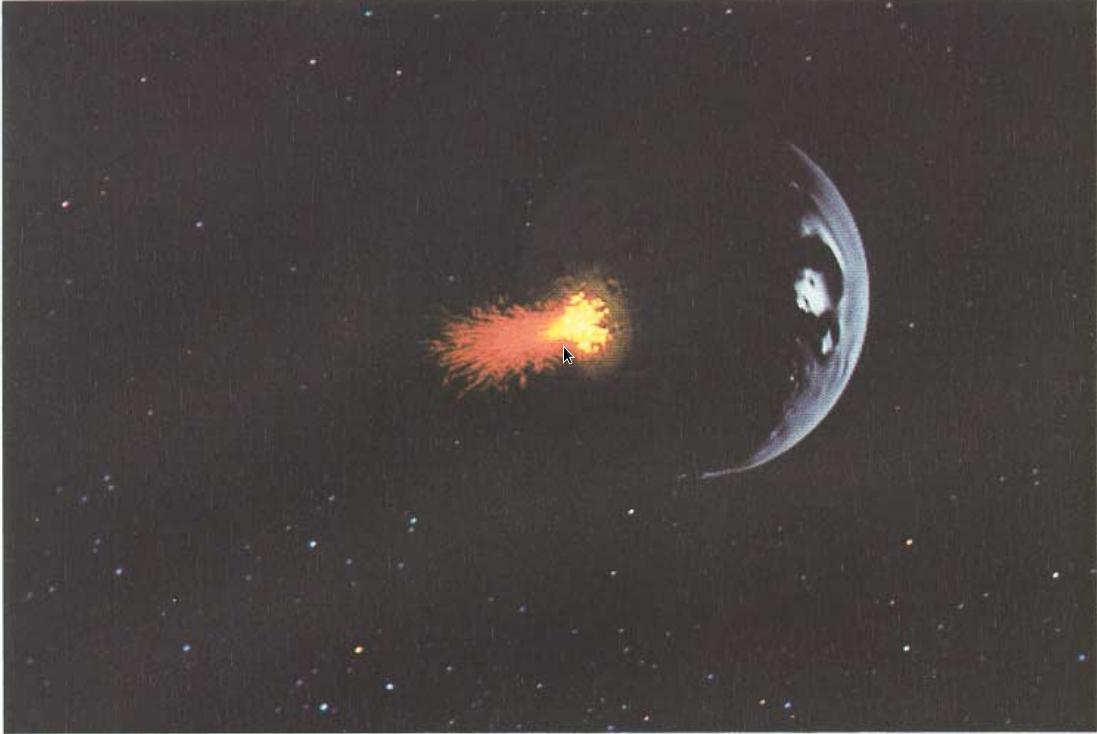
\includegraphics[width=\textwidth]{st2_init}
	\caption{Первоначальный взрыв}%
    \label{fig:reeves_1}
\end{figure}
\begin{figure}[htb]
	\centering
	
\includegraphics[width=\textwidth]{st2wall}
	\caption{Стена огня вот-вот поглотит камеру}%
    \label{fig:reeves_2}
\end{figure}
Система частиц верхнего уровня находилась в центре взрыва генезис-бомбы, она
генерировала частицы, которые в свою очередь являлись системами частиц.  Эти
системы частиц использовались для моделирования взрывов, при которых каждая
такая система частиц вела себя как небольшой вулкан, извергающийся в сторону
распространения взрывной волны и затухающий под воздействием силы гравитации.
Поскольку частицы имеют дискретную природу, для достижения хороших результатов
потребовалось колоссальное количество частиц. Но, поскольку моделирование в
реальном времени не требовалось, это не оказалось проблемой.

\subsection{Оффлайн симуляция}
В данное время наибольшего успеха исследователи добились в нечувствительном к
времени симуляции кинематографе. Несмотря на то, что данная работа нацелена на
компьютерную графику реального времени, необходимо упомянуть несколько работ в
области оффлайн симуляции, поскольку понимание основных идей, заложенных в них,
позволил перенести некоторые из них в область графики реального времени.

В публикации 2002 года Nguen и его коллеги представили метод моделирования огня,
полностью основанный на физико-математическом подходе~\cite{nguen2002}. В
симуляции использовались несжатые уравнения Навье-Стокса для горячих газов, это
позволило также смоделировать эффект расширения, вызванный испарением, и эффект
текучести поднимающихся дыма и сажи (рис.~\ref{fig:nguen}).
\begin{figure}[htb]
	\centering
	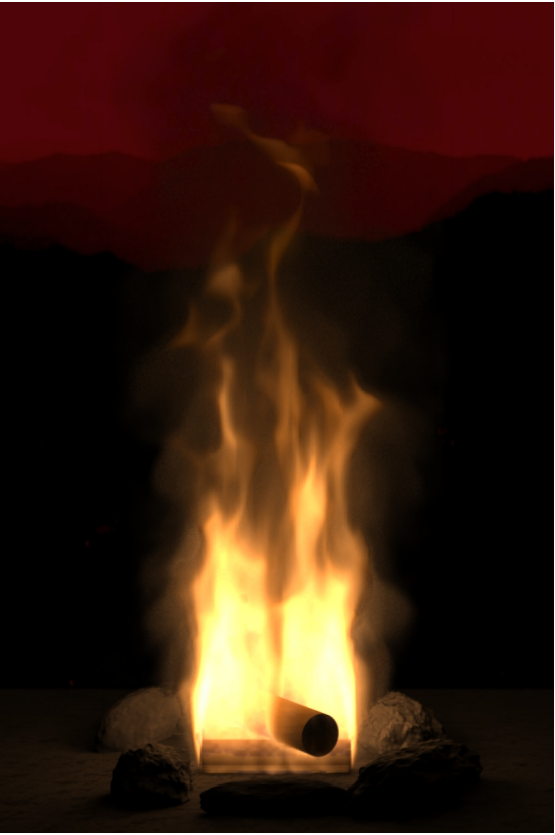
\includegraphics[width=0.4\textwidth]{nguen1}
    \caption{Два горящих полена находятся на земле и являются источником
    топлива. Бревно, лежащее поперек, еще не загорелось, поэтому пламя его
обтекает}%
    \label{fig:nguen}
\end{figure}
Как видно на изображении, данная симуляция отличается реалистичным
позиционированием и движением газообразных субстанций.  Однако данный подход
сложно реализовать в рендеринге реального времени, поскольку необходимо находить
решение большого количества комплексных уравнений за время кадра.

В 2008 году Horwath H\@. и Geiger W\@. представили инновационную комбинацию
симуляции с помощью крупной решетки частиц и тонко настроенных
визуально-ориентированных улучшений симуляции, рассчитываемых на
GPU~\cite{Stock:2008:SWF:1400385.1400457}. Полученные изображения имеют
поразительную детализацию и могут быть легко интегрированы в кинематографические
фотоснимки (рис.~\ref{fig:gpu2008}).

Данная техника улучшения симуляции использует особенности и ограничения
зрительного восприятия, а также особенности концентрации внимания зрителя.
Множество независимых GPU используются для быстрого увеличения качества
изображения, что позволяет достичь очень высокого разрешения.
\begin{figure}[htb]
	\centering
	
\includegraphics[width=\textwidth]{gpu2008}
	\caption{Три различных кадра симуляции огня. Быстро движущийся огненный
	шар с искрами. Извивающийся костер. Плотная стена дыма и огня.}%
    \label{fig:gpu2008}
\end{figure}

\subsection{Онлайн симуляция}
Трехмерный огонь, моделируемый в реальном времени, находит свое применение в
интерактивных приложениях. Среди интерактивных приложений можно выделить
компьютерные игры, в которых необходимость показывать взрывы появилась
практически с самого момента их появления (рис.~\ref{fig:earlyGames}).
\begin{figure}
    \centering
    \subfloat[\small{Огонь создан с помощью пререндеренного ядра
	битмапа, которое окружают светящиеся анимированные в реальном
времени частицы}]{{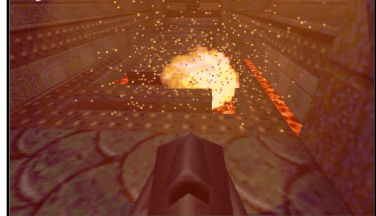
\includegraphics[height=4.0cm]{doom_splat} }}
    \qquad
    \subfloat[\small{Объемный факел, созданный из непрозрачных полигонов}]
    {{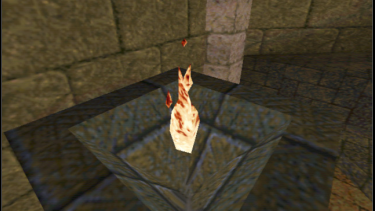
\includegraphics[height=4.0cm]{doom_torch} }}
    \caption{Скриншоты из Quake (1996)~\cite{capstone}}%
    \label{fig:earlyGames}%
\end{figure}
Компьютерные игры являются основными потребителями графических компьютерных
анимаций огня. Однако это стало возможным лишь пару десятилетий назад. С тех пор
скорость аппаратного обеспечения для рендеринга время росла экспоненциально,
открывая возможности для все более и более детализированных эффектов
(рис.~\ref{fig:farcry2}). К сожалению, поскольку игры зачастую являются
проприетарными по своей природе, литературных источников по алгоритмам,
используемых в играх крайне мало.
\begin{figure}[htb]
	\centering
	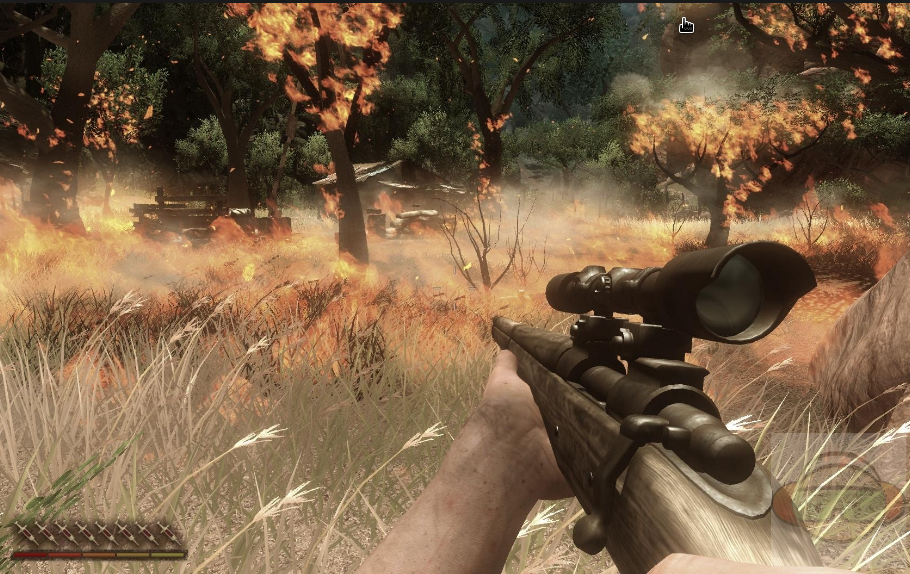
\includegraphics[scale=0.4]{farcry2}
	\caption{Far Cry 2 (2008)~\cite{farcry2}. На момент своего выхода в игре
	была наиболее реалистичная симуляция степных пожаров}%
    \label{fig:farcry2}
\end{figure}

Компания NVIDIA представила в 2014 году систему NVIDIA FlameWorks
(рис.~\ref{fig:FlameWorks}). Данная система позволяет добавлять реалистичный
огонь, дым и эффекты взрывов в игры.  Данная система совмещает передовую
симуляцию жидкостей на основе решетки вместе с эффективной системой объемного
рендеринга, все оптимизировано для работы в реальном времени. Все вычисления
выполняются на GPU с помощью DirectX 11~\cite{Green:2014:NFR:2633956.2658828}.
\begin{figure}[htb]
	\centering
	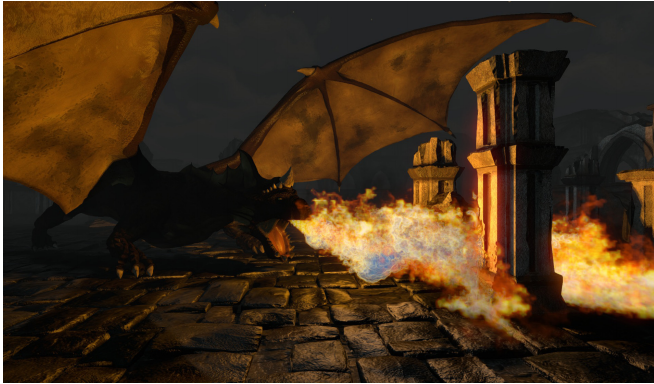
\includegraphics[width=\textwidth]{green2014}
	\caption{Демонстрация работы NVIDIA FlameWorks}%
    \label{fig:FlameWorks}
\end{figure}

Из опубликованных работ по симуляции огня в режиме реального времени можно
выделить работу~\cite{turbulence}. В данной работе представлена система, которая
предназначена для использования 3d-художниками. Пользователь может задать форму
пламени на различных этапах в виде рисунка, система производит расчет
промежуточных кадров и позволяет экспортировать результаты для рендеринга в
графических редакторах. Данный метод использует в качестве модели частицы,
рендеринг осуществляется с помощью сплайнов. Данный алгоритм развивает идеи,
предложенные ранее в~\cite{Vanzine2007RealisticRR}.

В работах~\cite{Zhao2003VoxelsOF}, описывается симуляция огня с помощью
вокселей. Данный метод позволяет достичь высокий уровень взаимодействия огня с
окружающей средой и объектами (рис.~\ref{fig:voxelFire}).  Данный метод
позволяет реализовать уничтожение огнем объектов из определенных материалов.
Недостатком данного метода является необходимость использования большого
количества памяти для хранения данных о вокселях.
\begin{figure}[htb]
	\centering
	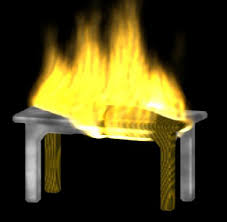
\includegraphics{voxels_on_fire}
    \caption{Воксельное пламя из~\cite{Zhao2003VoxelsOF}}%
    \label{fig:voxelFire}
\end{figure}

\section{Обзор и классификация алгоритмов симуляции огня}

Различные методы применяемые при симуляции огня можно условно разделить на
следующие группы:
\begin{itemize}
	\item текстурный маппинг;
	\item система частиц;
	\item физико-математические методы;
	\item клеточные автоматы;
	\item томографическая реконструкция и др.
\end{itemize}

В работе~\cite{realistic_sim} представлен различных техник для создания
реалистичной симуляции огня. В данной работе проанализировано несколько техник
симуляции огня, включая симуляцию с помощью вокселей и симуляцию с помощью
стабильных флюидов. Приведено кратное описание каждой техники, с описанием их
преимуществ и недостатков.

В 2011 году ZhaoHui W., Zhong Z. и Wei W. представили статью~\cite{survey}, в
которой проанализировали современные алгоритмы симуляции реалистичного огня. Ими
был проведен анализ наиболее популярных методов по следующим критериям:
\begin{itemize}
	\item применимость в реальном времени;
	\item степень реалистичности;
	\item пространственно-временная сложность;
	\item конфигурируемость;
	\item интерактивность.
\end{itemize}
Результаты данного исследования можно увидеть в таблице~\ref{table:algoAnalsysis}.

\begin{table}[htb]
    \caption{Сравнение производительности различных методов симуляции огня}
    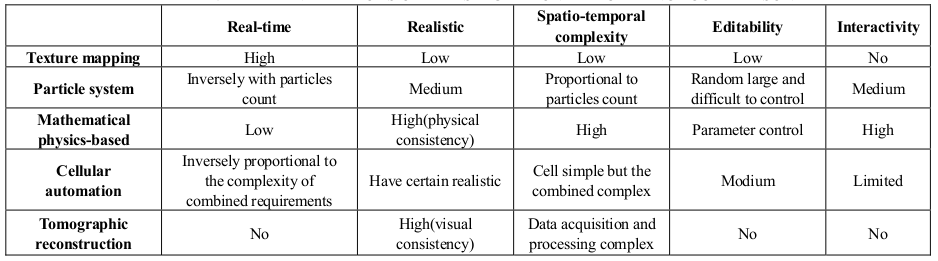
\includegraphics[width=\textwidth]{simulation_methods}%
    \label{table:algoAnalsysis}
\end{table}

\textbf{Выводы по главе 1:}
\addcontentsline{toc}{section}{Выводы по главе 1}
\begin{enumerate}
    \item При выборе алгоритма для динамической симуляции необходимо найти
        баланс между реалистичностью симуляции и скоростью симуляции. Частота
        кадров не должна падать ниже заданного минимального уровня.
    \item Моделирование огня с помощью системы частиц до сих пор является
        наиболее популярным методом, который позволяет обеспечить средний
        уровень реалистичности, но при небольшом количестве частиц обеспечивает
        высокую скорость симуляции. Данный метод будет использован для
        моделирования частиц в рамках диссертации.
    \item Для расчета параметров анимации огня в диссертации будут использованы
        уравнения Навье-Стокса, поскольку они позволяют получить крайне
        реалистичную анимацию. Для борьбы с высокой сложностью расчетов в
        дальнейшем будет выбран оптимальный числовой метод, который позволит
        получить решение с достаточной точностью, сохранив при этом приемлемую
        частоту кадров.
    \item В качестве примитива для рендеринга в разрабатываемой системе будут
        использованы воксели. Воксельная графика позволяет получить визуально
        реалистичное изображение, также упроститься реализация взаимодействия
        огня с окружающими объектами. Для уменьшения требований к аппаратным
        ресурсам будут использованы оптимизационные алгоритмы, которые позволят
        уменьшить количество примитивов для отрисовки.
\end{enumerate}


\chapter{Теория динамической симуляции огня}

В данной главе будут приведены основные теоретические сведения, которые
необходимы для введения в практическую часть диссертации. В главе будут
приведены необходимые определения из областей компьютерной графики, физики
математической симуляции, будут представлены рисунки и уравнения, поясняющие
информацию.

Глава состоит из трех разделов:
\begin{enumerate}
    \item В разделе ''Теория компьютерной графики'' приводятся определения
        терминов из области компьютерной графики, которые будут использоваться
        далее в тексте диссертации. Также в раздели приведен обзор преимуществ и
        особенностей библиотеки OpenGL, которая будет использована для создания
        практической части диссертации.
    \item Раздел ''Физика огня'' описывает огонь как физический процесс. В
        разделе будет дано описание процесса горение, приведено отличие между
        терминами ''огонь'' и ''пламя'', дано объяснение некоторым особенностям
        внешнего вида и поведения огня.
    \item В разделе ''Динамическая симуляция огня'' можно найти описание\break{}
        структуры симуляции огня и ее элементов. Каждая из задач симуляции будет
        подробно описана. В разделе присутствует описание преимуществ и
        недостатков популярных алгоритмов в области динамической симуляции огня.
\end{enumerate}.

\section{Теория компьютерной графики}

\subsection{Введение в компьютерную графику}

Для начала необходимо дать определение компьютерной (или машинной) графике.

\textbf{Компьютерная графика} --- это совокупность технических, математических и
программных средств и приемов, позволяющих осуществлять ввод и вывод из ЭВМ
графической информации без ручного преобразования информации в числовую или
графическую форму~\cite{SamalGraphics}.

Можно выделить три основных этапа формирования изображения электронной
вычислительной машиной:
\begin{itemize}
    \item построение модели объекта или сцены, содержащей несколько объектов
        (т\@.е\@. описание объектов и их связей в рамках евклидовой геометрии);
    \item подготовка модели к визуализации в зависимости от местонахождения
        наблюдателя (выполнение геометрических преобразований, удаление
        невидимых линий);
    \item визуализация с помощью заданного устройства отображения (отсечение по
        объему/окну видимости, формирование растрового представления, наложение
        текстуры, затенение, добавление дополнительных эффектов, вывод на
        терминал).
\end{itemize}

Изображение можно представить в виде множества точек, линий, строк текста и
закрашенных областей, называемых \textbf{примитивами}. При этом изображение чаще
всего описывается набором вершин, ребер и граней, формирующих в итоге множество
прямоугольников с заданными атрибутами и представляющих в совокупности один или
несколько объектов сцены. Следует отметить, что визуализация изображений, как
правило, выполняется на плоскости, т\@.е\@. итоговое изображение двухмерно, и,
таким образом, при отображении трехмерных объектов одним из обязательных шагов
является проективное преобразование.

Периферийные устройства вывода делятся по своему типу на растровые и векторные.
В настоящее время визуализация изображений производится в большинстве случаем
именно растровыми устройствами вывода. В растровых устройствах отображения точку
заменяет пиксель (от английского \textit{picture element}). \textbf{Пиксель} ---
это наименьшая часть изображения, с которой может работать алгоритм обработки
либо визуализации изображения.

Изображения, отображаемые на растровых устройствах, либо хранимые в виде
двухмерного массива значений пикселей --- растра, называются
\textbf{растровыми}. Процесс преобразования векторных моделей в растровые
изображения называется \textbf{растеризацией}.

\subsection{Библиотека OpenGL}

В практической часть диссертации для создания трехмерной (3D) графики
используется библиотека OpenGL\@. \textbf{OpenGL} --- это программный интерфейс,
который позволяет приложениям пользоваться и управлять графической подсистемой
устройства, на котором работает OpenGL~\cite{OGLSuperbible}.

OpenGL может работать на различных устройствах от дорогостоящих профессиональных
рабочих станций до обычных настольных компьютеров, от игровых консолей до
мобильных телефонов. OpenGL предлагает стандартизированный интерфейс (API),
который предоставляет широкую портируемоесть и позволяет разработчикам
приложений фокусировать свое внимание на создании качественных продуктов,
разработке интересного контента, и увеличении производительности своих
приложений вместо того, чтобы беспокоиться о спецификациях платформы, для
которой они создают приложение.

OpenGL может разбивать поток работы на фундаментальные элементы и выполнять их
параллельно. Комбинации конвейеризации и параллелизма позволяет получить
максимальную производительность от современных графических процессоров.
Структура графического конвейера представлена на
рисунке~\ref{fig:graphicsPipeline}.
\begin{figure}[htb]
	\centering
	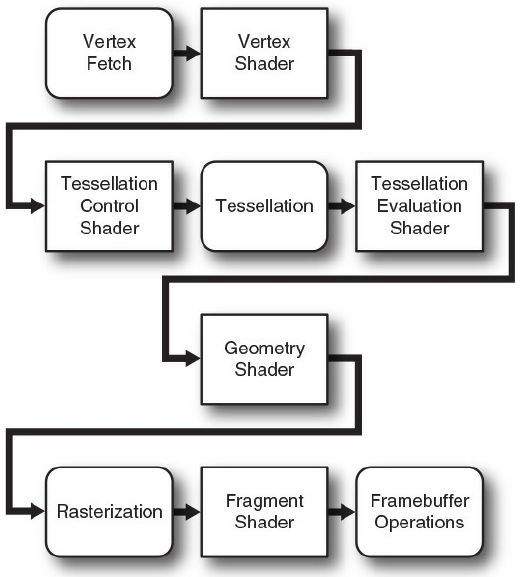
\includegraphics[width=0.75\textwidth]{graphicsPipeline}
	\caption{Упрощенная структура графического конвейера}%
    \label{fig:graphicsPipeline}
\end{figure}
На рисунке~\ref{fig:graphicsPipeline} блоки со скругленными краями представляют
собой фиксированные части, которые обычно реализованы как часть драйвера,
прошивки или другого системного ПО. Блоки с прямоугольными краями являются
программируемыми, это означает, что они могут выполнять шейдеры, предоставляемые
разработчиками ПО.

На момент написания диссертации существует 20 изданий спецификации
OpenGL~\cite{OpenGLHistory}. Номера версий и даты их публикации приведены в
таблице~\ref{table:OpenGLVersions}.
\begin{table}
\caption{Версии OpenGL}%
\label{table:OpenGLVersions}
\centering
\small
\begin{tabular}{| l | l |}
    \hline
    Версия & Дата публикации \\
    \hline
    OpenGL 1.0 & Январь 1992 \\
    OpenGL 1.1 & Январь 1997 \\
    OpenGL 1.2 & Март 1998 \\
    OpenGL 1.2.1 & Октябрь 1998 \\
    OpenGL 1.3 & Август 2001 \\
    OpenGL 1.4 & Июль 2002 \\
    OpenGL 1.5 & Июль 2003 \\
    OpenGL 2.0 & Сентябрь 2004 \\
    OpenGL 2.1 & Июль 2006 \\
    OpenGL 3.0 & Август 2008 \\
    OpenGL 3.1 & Март 2009 \\
    OpenGL 3.2 & Август 2009 \\
    OpenGL 3.3 & Март 2010 \\
    OpenGL 4.0 & Март 2010 \\
    OpenGL 4.1 & Июль 2010 \\
    OpenGL 4.2 & Август 2011 \\
    OpenGL 4.3 & Август 2012 \\
    OpenGL 4.4 & Июль 2013 \\
    OpenGL 4.5 & Август 2014 \\
    OpenGL 4.6 & Октябрь 2017 \\
    \hline
\end{tabular}
\end{table}
Старые версии OpenGL предлагали непосредственный режим работы (фиксированный
конвейер), который был простым способом для отрисовки графики.
Однако, большинство функционала было спрятана в библиотеке и у разработчиков не
было большого контроля над вычислениями. Начиная с версии 3.2 спецификации
началось стимулирование перехода разработчиков к новому API (core профиль),
который является версией спецификации, в которой убрана вся устаревшая
функциональность. Начиная с версии 3.3 радикальных изменений в спецификации не
происходило, в последующих версиях были добавлены некоторые функции для более
удобного выполнения частых задач. Разработанная в ходе диссертации система
использует спецификацию OpenGL версии 4.5, однако может быть легко портирована и
на более ранние версии.

Необходимо вернуться к обзору графического конвейера и дать определение понятию
''шейдер''. \textbf{Шейдеры} --- это небольшие программы, которые предназначены
для выполнения на графическом процессоре~\cite{LearnOGL}. Шейдеры могут
одновременно выполняться на тысячах вычислительный ядер ГП. Для вывода
изображения на экран необходимо наличие в шейдерной программе как минимум
вершинного и фрагментного шейдеров. Для написания шейдеров на OpenGL
используется \textbf{OpenGL Shading Language (GLSL)}. GLSL\@--- Си-подобный язык,
который также является частью спецификации OpenGL\@.

Одну из особенностей OpenGL является использование пяти различных координатных
систем:
\begin{itemize}
    \item локальное пространство (или пространство объекта);
    \item мировое пространство;
    \item пространство наблюдателя;
    \item пространство отсечения;
    \item экранное пространство.
\end{itemize}

Для преобразования координат из одного пространства в другое, используется
несколько различных матриц трансформации, среди которых, самыми важными являются
матрицы модели, вида и проекции. Координаты вершин появляются в локальном
пространстве как локальные координаты, и в дальнейшем преобразуются в мировые
координаты, потом в координаты вида, отсечения, и, наконец, все все координаты
приводятся к экранному пространству. На рисунке~\ref{fig:spaceTransforms}
представлена вся последовательность преобразований и эффект, который оказывает
каждое преобразование:
\begin{figure}[htb]
	\centering
	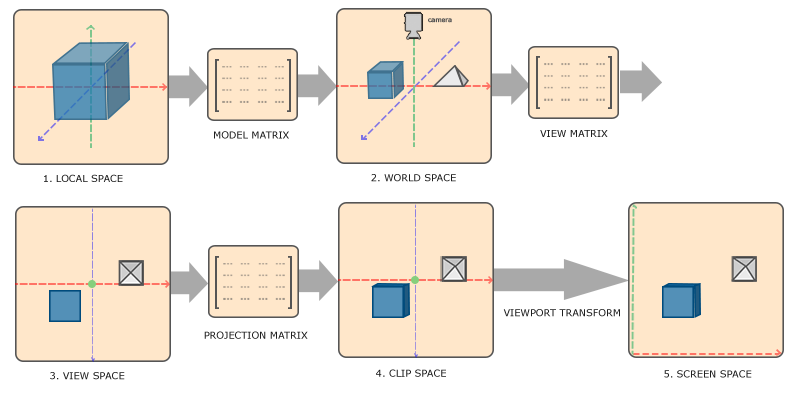
\includegraphics[width=\textwidth]{spaceTransforms}
	\caption{Преобразования систем координат в OpenGL}%
    \label{fig:spaceTransforms}
\end{figure}
\begin{enumerate}
    \item Локальные координаты это координаты объекта измеряемые относительно
        точки отсчета расположенной в центре объекта.

    \item На следующем шаге локальные координаты преобразуются в координаты
        мирового пространства, которое содержит все объекты сцены. Эти
        координаты измеряются относительно глобальной точки отсчета, единой для
        всех объектов расположенных в мировом пространстве.

    \item Далее происходит преобразование мировых координаты в координаты
        пространства наблюдателя таким образом, что каждая вершина становится
        видна как если бы на нее смотрели из камеры или из местоположения
        наблюдателя.

    \item После того, как координаты были преобразованы в пространство
        наблюдателя, необходимо спроецировать их в координаты пространства
        отсечения. Координаты пространства находятся в диапазоне от -1.0 до 1.0
        и определяют, какие вершины появятся на экране.

    \item И, наконец, происходит преобразование координат в экранное
        пространство. Размер пространства определяется размером окна, в котором
        происходит рендеринг изображения. В качестве точки отсчета берется
        нижний левый угол окна. Полученные координаты отсылаются растеризатору
        для превращения их во фрагменты (пиксели).
\end{enumerate}

Операцию приведения координат из пространства в модели в пространство отсечения
можно выполнить с помощью формулы (\ref{eq:mvp}).
\begin{equation}
  \label{eq:mvp}
  \text{V}_\text{clip} = \text{M}_\text{proj} \cdot \text{M}_\text{view} \cdot
  \text{M}_\text{model} \cdot \text{V}_\text{local}
\end{equation}
\begin{explanationx}
    \item [где] $\text{V}_\text{clip}$ --- координаты вершины в пространстве
        отсечения;
    \item $\text{M}_\text{proj}$ --- матрица преобразования в пространство
        отсечения;
    \item $\text{M}_\text{view}$ --- матрица преобразования в пространство
        наблюдателя;
    \item $\text{M}_\text{model}$ --- матрица преобразования в мировое
        пространство;
    \item $\text{V}_\text{local}$ --- координаты вершины в локальном
        пространстве.
\end{explanationx}

Матрицы не обладают свойством коммутативности, поэтому важно выполнять умножение
в правильном порядке. Умножение матриц следует читать в обратном порядке,
т\@.к\@. сначала к вершине применяется самая правая операция.

\section{Физика огня}

Перед тем, как приступить к симуляции огня, нужно глубже разобраться в природе
исследуемого объекта. Необходимо выделить разницу между огнем и пламенем,
дать определение процессу горения и описать его компоненты, сделать обзор
основных видов огня и глубже разобраться в физике процесса горения.

\subsection{Компоненты горения}

В разговорном русском языке нет четкого смыслового разделения между словами
''пламя'' и ''огонь''\cite{WikiFlame}, однако в зарубежной литературе
присутствует четкое разделение понятий огонь (fire) и пламя (flame). Также в
некоторых технических русскогоязычных словарях приводится трактовка этих
понятий.

Несмотря на то, что стандарт СТ СЭВ 383--87~\cite{383-87} уже устарел, в нем
дается точное определение для ключевых терминов, используемых в диссертации. В
следующих подразделах также будут приведены определения из данного стандарта.

\textbf{Огонь} --- процесс горения, сопровождающийся пламенем или свечением.

\textbf{Пламя} --- зона горения в газовой фазе с видимым излучением.

Среди процессов химических веществ бывают случаи, когда вещество сгорает без
пламени~\cite{WikiFire}.

Обычно люди воспринимают горящий объект, словно объект горит сам по себе.
Однако, на самом деле пламя образует не сам объект, а топливо, которое он
выделяет в окружающую среду. Топливо подымается над поверхностью объекта из-за
тепла, испаряется, вступает в контакт к кислородом и воспламеняется. Таким
образом, огонь нуждается в совместном присутствии трех элементов: топливо, тепло
и кислород~\cite{USArmy}:
\begin{enumerate}
    \item \emph{Топливо}. Топливом может быть твердая, жидкая либо газообразная
        субстанция, также топливо должно химически разлагаться на газы или
        пар. Процесс разложения происходит под воздействием тепла.
    \item \emph{Тепло}. Тепло --- это мера молекулярной активности в объекте,
        увеличение температуры ведет к увеличению скорости движения молекул.
        Если к объекту приложено достаточно тепла, молекулы начинают двигаться
        настолько быстро, что могут покидать поверхность объекта. Так происходит
        процесс перехода топлива в газообразное состояние.
    \item \emph{Кислород}. Кислород является окисляющим агентом и поэтому
        необходим для процесса горения. На определенном уровне, частицы огня
        могут превращаться в частицы дыма из-за нехватки кислорода в воздухе,
        что вызывает неполное окисление.
\end{enumerate}

\subsection{Воспламенение объектов}

\textbf{Горение} --- экзотермическая реакция окисления вещества,
сопровождающаяся по крайней мере одним из трех факторов: пламенем, свечением,
выделением дыма~\cite{383-87}.

Процесс горения имеет следующие стадии:
\begin{enumerate}
    \item Окисление вызывает разложение горючего материала, происходит\break{}
        медленное выделение газов, включая водяной пар.  Процесс протекает
        непрерывно все время, в течение которого объект взаимодействует с
        окисляющим агентом, которым может выступать кислород. При температуре
        окружающей среды окисление обычно происходит настолько медленно, что
        даже незаметно человеку. Горючие газы пока еще не могут воспламенятся на
        этой стадии.

    \item Скорость окисления возрастает с ростом температуры, в это время
        некоторые газы становятся воспламеняемыми. Точка, когда в воздухе
        находится достаточное количество пара, чтобы создать горючую смесь в
        воздухе, называется \emph{точкой вспышки}.

    \item В вышеупомянутой точке в выделенных газах присутствует слишком много
        углекислого газа и водяного пара, чтобы поддерживать пламя
        продолжительное время. Однако, тепло огня служит началом для вторичного
        процесса разложения, которое приводит к процессу устойчивого горения.
        Эта точка называется \emph{точкой воспламенения}, и она обычно находится
        на несколько градусов выше точки вспышки.

    \item Окисление может идти настолько быстро, что оно покрывает всю
        поверхность топлива и блокирует доступ к кислороду, препятствуя горению
        топлива и затрудняя проникновение тепла. Это задерживает распространение
        температуры воспламенения вглубь горючего материала. Однако, с
        увеличением температуры топливо начинает светиться, воздух поступает
        внутрь для поддержания горения, и происходит горение топлива совместно с
        выделяемыми газами.

    \item Если тепла выделяется больше, чем теряется из-за проводимости,
        конвекции или излучения, огонь будет поддерживаться и появится пламя.
        Горение будет поддерживаться, пока либо тепло, горючее, или окисляющий
        агент не будут убраны из системы.
\end{enumerate}

\subsection{Классификация огня}

Следуя классификации, предложенной в~\cite{nielsen}, огонь может быть разделен
по визуальным характеристикам на следующие группы:
\begin{enumerate}
    \item \emph{Спокойный огонь}. Типичным примером спокойного огня
        является \break{} огонь свечи. Спокойный огонь редко нарушается
        воздействием внутренних либо внешних сил. Таким образом, огонь остается
        спокойным и практически не движется, если движется вообще.

    \item \emph{Свободно питаемый огонь}. Свободно питаемый огонь не
        испытывает нехватки топлива и получает достаточное количество кислорода,
        также количество топлива и кислорода варьируется в зависимости от
        времени и местоположения. Это существенно отличается он спокойного огня,
        который имеет более или менее постоянное и контролируемое количество
        топлива и доступного кислорода на протяжении всего времени горения и во
        всех областях огня.

    \item \emph{Сильный огонь}. В сильном огне, внешние силы оказывают сильное
        влияние на огонь, вызывая неравномерную подпитку огня и распространение
        топливных компонентов в направлениях, отличных от вертикального. Сильный
        огонь крайне переменчив и крайне непредсказуем из-за сложности лежащих в
        его основе систем и большого количества влияющих сил.

    \item \emph{Огонь, подаваемый под давлением}. Огонь, подаваемый под
        давлением --- это свободный огонь, вектора скорости которого направлены
        в сторону, в которую происходит выброс топлива в воздух.

    \item \emph{Детонации и взрывы}. \emph{Взрыв} — это процесс, в котором за
        короткое время в ограниченном объёме выделяется большое количество
        энергии и образуются газообразные продукты взрыва, способные совершить
        значительную механическую работу или вызвать разрушения в месте
        взрыва~\cite{WikiDetonation}. В \emph{детонациях} используется изначально
        сжатое топливо; возгорание вызывает взрывную волну, которая вызывает
        серию небольших взрывов, которые создают новые взрывные волны.
\end{enumerate}

Также хочется отметить такой процесс, как пожар. \textbf{Пожар} ---
неконтролируемое горение, приводящее к ущербу. При моделировании пожаров
основной упор делается на расчет скорости распространения дыма и огня, вместо
реалистичной визуализации зачастую используется схематичная. Моделирование
пожаром находится за пределами данного исследования.

\subsection{Визуальное восприятие огня}%
\label{section:firePerception}

Огонь является довольно сложным природным феноменом. В данном подразделе будет
приведен обзор основных физических особенностей, влияющих на визуальное
восприятие человеком огня. В данном разделе будут приведены моменты касательно
спектра огня, сопротивления воздуха, вызывающего эффект подергивания,
формирования и вида сажи и дыма.

Обычно в естественных науках огонь рассматривают в качестве излучателя черного
тела, для описания цвета. Черное тело испускает фотоны различных цветов, от
черного до белого, проходя через красный, оранжевый и желтый. Цветовой спектр
излучения черного тела приведен на рисунке~\ref{fig:fireSpectrum}. Данный спектр
несколько ограниченно описывает световое излучение, испускаемое в процессе
горения, поскольку он не учитывает вклад различных примесей, которые могут
сильно влиять на цвет пламени.
\begin{figure}[htb]
	\centering
    
\includegraphics[width=0.75\textwidth]{fireSpectrum}
	\caption{Спектр излучения черного тела}%
    \label{fig:fireSpectrum}
\end{figure}

Взаимодействие цвета и температуры можно рассмотреть на примере горения свечи,
представленной на рисунке~\ref{fig:candle}.
\begin{figure}[htb]
	\centering
    
\includegraphics[width=0.4\textwidth]{candle}
	\caption{Горение свечи}%
    \label{fig:candle}
\end{figure}
Часть пламени, наиболее близкая к фитилю, невидима, изменяясь постепенно к
голубоватому цвету на границе и у основания пламени. В самой горячей точке пламя
приобретает белый цвет. Остальные регионы пламени имеют светло-желтый цвет,
который постепенно переходит в оранжевый или красный у вершины. Быстрое
сравнение цветов пламени свечи и цветовой палитры излучения черного тела
показывает ограничения палитры, поскольку она не нацелена на отображение пламени
на восковом топливе.

Необходимо также описать факторы, влияющие на движение огня. Следующий пример,
иллюстрирующий движение горячего турбулентного газа был взят
из~\cite{Foster1997ModelingTM}. Представим старомодный паровой двигатель,
выпускающий\break{}струю горячего пара из своего бойлера. В самом начале,
ведущим фактором, влияющим на движение газа, является скорость, с которой его
выпустили в окружающую среду. В то время, как пар смешивается с более медленно
двигающимся воздухом, пар испытывает \emph{сопротивление воздуха} (drag), и
начинает вращаться в некоторых местах. Это вращение усиливает смешивание с
воздухом и вызывает появление завихрений, которые мы можем наблюдать при
смешивании газов. Согласно~\cite{Foster1997ModelingTM}, следующим важным
фактором, влияющим на движение газа является температура. Как только струя пара
была выпущена, она поднимается вверх, и более горячие участки подымаются
быстрее, чем области, которые смешались с более холодным воздухом. В то время,
как газ подымается, он испытывает внутреннее сопротивление воздуха, которое
создает еще больше турбулентного вращения. Этот эффект известен под названием
\emph{термальной плавучести} (thermal buoyancy). Влияние сопротивления воздуха и
термальной плавучести на движение газов приведено на
рисунке~\ref{fig:gasMotion}.
\begin{figure}[htb]
	\centering
    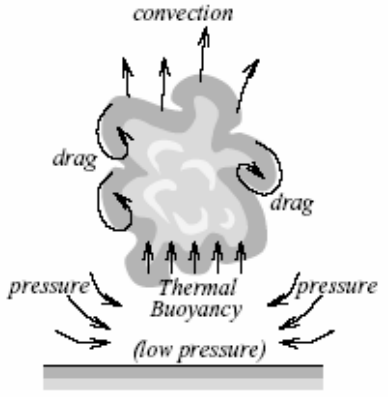
\includegraphics[width=0.4\textwidth]{gasMotion}
	\caption{Движение горячего газа}%
    \label{fig:gasMotion}
\end{figure}

Наконец, дым и сажа появляются при недостатке в ядре огня кислорода для
поддержания процесса горения. На выходе получается неполное сгорание, которое
производит такие побочные продукты как сажа. Дым является результатом смешивания
сажи с водой, что обычно происходит в процессе горения. Дым от огня зачастую
очень темный из-за высокого содержания углекислого газа в воздухе. Однако, из-за
влияния различных компонентов горючего материала или других побочных продуктов
горения, в воздух могут подыматься примеси и других цветов. Например, пар имеет
серый цвет (количество воды преобладает над количеством сажи).

\section{Особенности рендеринга в реальном времени}

В~\cite{Young1982RealTL} приводится определение системы реального времени как
''системы, которой необходимо отвечать на внешние входные данные за конечный и
определенный период.'' Таким образом, симуляция огня в режиме реального времени
--- это симуляция, поведение и окружение которой должно быть рассчитано за
период времени, соизмеримый с ее поведением и окружением в реальном мире. Это
отличается от конвейера, используемого в оффлайн симуляции при производстве
фильмов, где расчет каждого кадра может занимать минуты либо часы.

В общем случае, в компьютерной графике существует большой отрыв между скоростью
и реализмом. В приложениях реального времени наибольший приоритет отдается
скорости. Таким образом, ключевой проблемой симуляции в реальном времени
является поиск баланса между количеством вычислений для достижения оптимального
результата, не допуская при этом падения частоты кадров ниже минимальной
допустимой границы.

Для каждого желаемого атрибута необходимо выбрать оптимальный алгоритм для
конкретного случая. Такая оптимальность зачастую достигается внедрением
разнообразных ухищрений, которые имеют слабую связь с поведением объектов в
реальном мире, однако они позволяют достичь желаемого эффекта. Некоторые примеры
таких ухищрений будут описаны ниже в этом разделе. Суть идеи в том, что пока
симуляция показывает визуально приемлемые результаты и выполняется с достаточно
быстрой скоростью, скорее всего никто не заметит особых различий. Использование
таких ухищрений не является чем-то зазорным, поскольку они с самого присутствуют
в индустрии компьютерной графики с самого момента ее появления. По факту, на
момент своего появления вся индустрия компьютерной графики сплошь состояла из
таких ухищрений.

В общем случае задача симуляции огня может быть разбита на три
непересекающихся подзадачи~\cite{Perry94synthesizingflames}:
\begin{itemize}
	\item моделирование;
	\item анимация;
	\item визуализация.
\end{itemize}

В первую очередь необходимо выбрать подходящую внутреннюю структуру, или модель,
для симуляции. Далее, требуется выбрать способ анимации --- метод, с помощью
которого будет происходить взаимодействие с моделью. Техника анимации служит для
того, чтобы оживить модель, привести ее в движение. Наконец, модель и ее
анимацию необходимо отрисовать на экране, используя для этого некоторые
примитивы визуализации (полигоны, текстуры, сферы, воксели и т.п.).

Альтернативная схема была предложена в~\cite{realistic_sim}, в которой авторы
делают акцент на алгоритмах распространения огня. Фаза моделирования в данном
случае является одним из этапов при разработке алгоритмов распространения
огня. Схема, предложенная в данной работе, представлена на
рисунке~\ref{fig:simStages}.

\begin{figure}[htb]
	\centering
    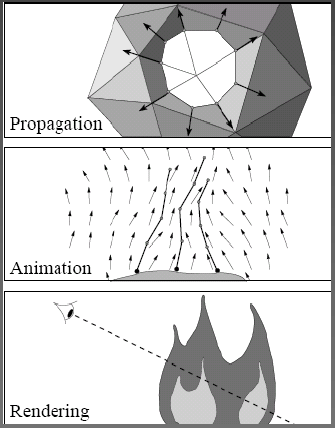
\includegraphics[width=0.4\textwidth]{simStages}
    \caption{Структура симуляции, предложенная в~\cite{realistic_sim}}%
    \label{fig:simStages}
\end{figure}

Более подробный обзор каждой стадии симуляции будет основан на схеме,
предложенной в~\cite{realistic_sim}. В последующих подразделах будут
последовательно рассмотрены каждая из стадий симуляции, и будут описаны нюансы
их взаимодействия.

\subsection{Моделирование и визуализация огня}

Стохастические методы моделирования огня, такие как поля турбулентности и шумов
очень эффективны при создании реалистичного огня в 2D графике, но являются
крайне неэффективными по количеству операций для использования в 3D анимациях в
реальном времени, независимо от выбранной техники визуализации. Альтернативой
может быть эффективно реализованная объемная модель рендеринга, использующая
воксели в качестве примитива визуализации, помогает достичь приемлемую для
интерактивных приложений частоту кадров. Однако, при использовании данной модели
сложно добиться реалистичных результатов, поскольку поверхность огня не имеет
четких границ. Наиболее быстрым методом является объемное моделирование с
использованием полигонов для визуализации; отрисовка полигонов происходит крайне
быстро, однако полигоны не лучшее средство для визуализации языков пламени,
вихрящегося дыма и частиц сажи, и поэтому обычно полигоны пораждают довольно
грубые и низкокачественные результаты. Где-то между ними находится моделирование
с помощью систем частиц, данный метод может работать с желаемой скоростью, в
зависимости от выбранного масштаба, который выбирается из расчета необходимого
уровня детализации и выбранных техник анимации и визуализации. Как было описано
в обзоре литературы, большинство симуляций огня используют системы частиц того
или иного вида. Этот метод также используется в практической части. Поэтому
дальнейшее описание симуляции будет сфокусировано на применении систем частиц.
Системы частиц позволяют моделировать трехмерное поведение огня в интуитивной и
простой манере, однако, они имею и свой набор недостатков, которые будут описаны
ниже.

Одной из проблем, связанных с системами частиц, является то, что они
предполагают одно и то же окружение для всех частиц в системе. Решением этой
проблемы является разбиение окружения на более мелкие части, называемые
\emph{полями}~\cite{nielsen}. Поле содержит информацию, касательно определенного
участка сцены, который зачастую представляет форму куба или прямоугольной
призмы, либо любой другой формы, которая может быть использована для создания
мозаики, описывающей окружение. Однако, поля оказывают большую нагрузку на
оперативную память. В идеальном случае, решетка должна охватывать всю сцену,
которая может быть подвержена влиянию огня, при этом ячейки должны иметь
достаточно малый размер, чтобы оказывать достаточно точное влияние на симуляцию.
Это является крайне сложной задачей для поиска оптимального решения, т\@.к\@.
установка всего лишь $10$ кубов в одном из измерений кубической сцены приводит к
$10^3 = 1000$ полей в сцене, при этом каждый кадр необходимо производить расчет
каждого поля. При этом, данная цифра является довольно заниженной оценкой,
поскольку окружение симуляции огня в основном имеет форму отличную от
кубической, и поэтому высота зачастую значительно превышает размеры ширины либо
глубины.

Второй проблемой систем частиц является то, что они требуют наличие огромного
количества частиц для полной симуляции системы, т\@.к\@. в идеальном случае
необходимо заниматься моделированием взаимодействий на молекулярном уровне.
Понятно, что задачу необходимо обобщить. \emph{Текстурный маппинг} является
одной из форм такого обобщения, и некоторые варианты данного метода является
часто используемым способом для достижения частоты кадров, необходимой при
симуляции в режиме реального времени. Пример текстурных карт представлен на
рисунке~\ref{fig:fireSplats}.
\begin{figure}[htb]
	\centering
    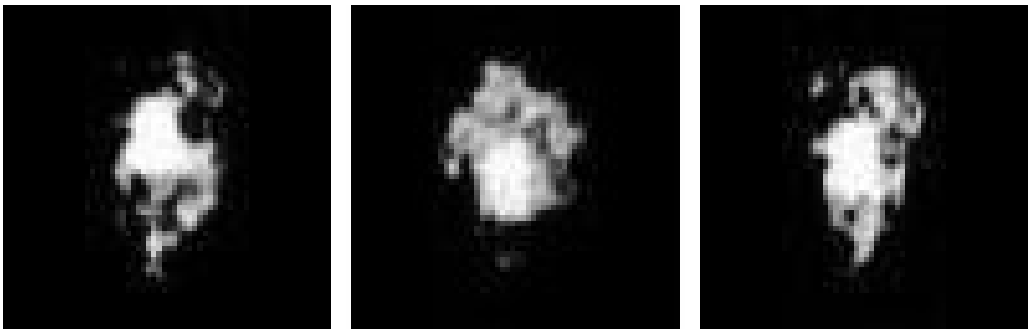
\includegraphics[width=0.5\textwidth]{fireSplats}
    \caption{Текстурные сплэты, созданные на основе
    фотографий~\cite{FireSplats}}%
    \label{fig:fireSplats}
\end{figure}
В методе текстурного маппинга статическая анимация огня накладывается на
полигоны, которые находятся на месте частиц в системе. Суть такого маппинга в
том, что теперь одна частица отображает целый кластер частиц, расположенных, как
на текстуре. Полигон обычно направлен на зрителя, когда тот перемещается по
сцене, с помощью вращения вдоль оси $y$. Однако, как можно заметить, в таком
случае полигон может быть направлен на зрителя только тогда, когда зритель
передвигается вдоль осей $x$ и $y$, и, как можно предположить, огонь будет
выглядеть довольно странно, если смотреть на него сверху, особенно сильно это
будет заметно, если посмотреть на сцену под острым углом. Еще одной проблемой,
связанная с использованием текстурного маппинга, является то, что освещение
сцены будет считать полигоны плоской поверхностью, и применять соответствующие
эффекты освещения к огню, которые, конечно, будут выглядеть крайне
нереалистично.

Одним из улучшений текстурного маппинга является текстурный сплэттинг, который
является техникой для симуляции объемного рендеринга. В текстурном сплэттинге
битовая карта складывается с картой прозрачности, таким образом битовая карта
становится частично прозрачной. Другими словами, текстурные приближения на
разных уровнях накладываются друг на друга с использованием смешивания.

Другим улучшением текстурного маппинга является использование
последовательностей изображений реального огня, вместо постоянного
переиспользования одной и той же текстуры для каждого полигона. Данное улучшение
помогает улучшить визуальное восприятие сцены с помощью уменьшения количества
статических элементов. Эта техника хорошо себя зарекомендовала и позволяет
получать довольно убедительные результаты.

Как можно заметить, метод текстурного маппинга позволяет успешно встраивать
заранее отрисованные элементы в симуляции в режиме реального времени. Так же
можно заметить, что при встраивании 2D текстур в 3D симуляцию, симуляцию уже
сложно назвать по-настоящему трехмерной. Однако, это является одним из тех
ухищрений, про которые шла речь в начале этого раздела. У текстур нет аналога в
реальном мире, поэтому это является своеобразным ухищрением. Текстуры слегка
смывают различие между 2D и 3D симуляцией, однако, использование текстур 2D
текстур в трехмерной симуляции довольно популярно, поскольку позволяет
существенно снизить вычислительную нагрузку. Разработанная в ходе исследования
система также использует данный прием.

\subsection{Анимация огня}

Существует множество способов анимации огня. Среди них можно выделить подходы,
использующие дифференциальные уравнения. Данные подходы позволяют получить
точные анимации, однако, они требуют отслеживания огромного числа переменных.
Производимые с помощью данных подходов симуляции тяжело контролировать,
поскольку их параметрами являются физические константы, чью взаимосвязь с
желаемыми визуальными характеристиками зачастую крайне сложно установить.
Вдобавок значения для этих параметров необходимо подбирать вручную, поскольку
природа огня еще до конца не изучена. Наиболее важно то, что эти подходы требуют
выполнения значительного количества вычислений, и поэтому их сложно применять в
симуляции в режиме реального времени.

Решением данной проблемы может быть попытка реализовать лишь наиболее важные
физические свойства огня, которые описаны в
разделе~\ref{section:firePerception}. Далее необходимо добиваться максимально
возможной реалистичности и\break{}эффектности каждого из компонентов. При этом
следует уделить внимание тому, чтобы реализация выглядела достаточно
правдоподобно и не была слишком уж заточена под конкретную сцену. Необходимо
стремиться к более элегантным решениям.

\textbf{Выводы по главе 2:}
\addcontentsline{toc}{section}{Выводы по главе 2}
\begin{enumerate}
    \item Для разработки практической части диссертации будет использована
        библиотека OpenGL\@. Core профиль OpenGL предоставляет большую
        свободу действий, что даст возможность тщательно реализовать и настроить
        различные атрибуты огня. Использование игровых движков является
        чрезмерным для данной задачи.
    \item В практической части диссертации будет выполняться симуляция свободно
        питаемого огня. Примерами такого огня в реальной жизни могут служить
        факел либо костер. Данный вид огня представляет интересную задачу для
        разработки анимации, и процессы, лежащие в его основе лучше поддаются
        математическому описанию, чем процессы, протекающие в сильном огне.
    \item Системы частиц будут использованы для моделирования огня. Для
        устранения недостатков данного метода будут применены различные приемы,
        такие как текстурный маппинг, рандомизация размеров, скорости и
        количества частиц.
    \item Анимация огня с помощью систем дифференциальных
        уравнений\break{}предъявляет высокие требования к аппаратным ресурсам и
        крайне сложно конфигурируется. Для создания анимации в рамках
        диссертации будут использованы более простые модели. Основной упор будет
        сделан на визуальное восприятие сцены.
\end{enumerate}



% Зачем: Изменение надписи для списка литературы
% Почему: Пункт 4.3.1 Положения о магистерской диссертации
\part*{Библиографический список}
\addcontentsline{toc}{part}{БИБЛИОГРАФИЧЕСКИЙ СПИСОК}
\addcontentsline{toc}{section}{Список публикаций соискателя}

\newrefcontext[labelprefix=A]
% \sloppy исправляет выходы за границы страницы
% https://tex.stackexchange.com/questions/118068/hyphenation-in-bibliography-with-biblatex
\sloppy\printbibliography[
    category=AuthorSources,
    heading=subbibliography,
    title={Список публикаций соискателя},
    resetnumbers,
]

\clearpage

\addcontentsline{toc}{section}{Список использованных источников}
\newrefcontext
\sloppy\printbibliography[
    notcategory=AuthorSources,
    heading=subbibliography,
    title={Список использованных источников},
    resetnumbers,
]
\clearpage


\addcontentsline{toc}{part}{Приложение Слайды презентации}

% \includepdf позволяет включить в результирующий pdf документ часть другого pdf документа, сделанного
% например не с помощью TeX. Бывает полезно, если какие-то диаграммны нарисованы, например, с помощью
% Microsoft Office и сохранены в pdf.

\includepdf[pages=1-4,
            pagecommand={
            \thispagestyle{plain}
            \hfill
            \begin{raggedleft}
                \begin{minipage}{5cm}
                    ПРИЛОЖЕНИЕ \\
                    Слайды презентации
                \end{minipage}
            \end{raggedleft}
            },
            nup=2x2,landscape=true,frame=true,
            noautoscale=true,scale=0.85,
            offset=1.0cm 0.0cm,delta=5mm 5mm]{build/presentation.pdf}


\includepdf[pages=5-last,
            pagecommand={\thispagestyle{plain}},
            nup=2x2,landscape=true,frame=true,
            noautoscale=true,scale=0.85,
            offset=1.0cm 0.0cm,delta=5mm 5mm]{build/presentation.pdf}


% \includepdf позволяет включить в результирующий pdf документ часть другого pdf документа, сделанного
% например не с помощью TeX. Бывает полезно, если какие-то диаграммны нарисованы, например, с помощью
% Microsoft Office и сохранены в pdf.

\includepdf[pages=1-last,
            pagecommand={\thispagestyle{plain}},
            nup=2x2,landscape=true,frame=true,
            noautoscale=true,scale=0.85,
            offset=1.0cm 0.0cm,delta=5mm 5mm]{build/presentation.pdf}

\end{document}
